\chapter{Reactor Design Verification}
    As discussed earlier, the scope of this project was not to develop a mature
reactor concept. Most of this work focused on modeling the mass of the
reactor as a function of flow inputs and thermal power requirements. It is
prudent however, to verify that the chosen reactor design is feasible as a
reactor concept. The purpose of this section is to convince the reader that
the chosen reactor design is valid, and with significant engineering effort,
could be developed into a working nuclear reactor. To this end, more detailed
neutronics modeling was performed on the chosen reactor design.

\section{Homogeneous Approximation}
All MCNP modeling was performed based on a homogeneous approximation for core
materials. The fuel, coolant, and cladding compositions were smeared to form a
single homogeneous core region. This approximation simplified the geometry which
helped automate the generation of thousands of input files for parametric
sweeps. A homogenous fuel mixture was deemed appropriate because there is little
moderation in the modeled systems. Average neutron energies are higher in the
absence of a moderator and higher energy neutrons have large mean free paths in
matter. This increased mean free path reduces the importance of small geometric
features.

The homogeneous approximation is known to be acceptable from decades of
experience modeling fast nuclear reactors. Still, it is important to check
assumptions. The homogeneous approximation was checked by comparing a
heterogeneous and a homogeneous \keff result for the same \uran mass and core
geometry. Coolant channels were added to the heterogeneous model and the fuel
fraction of the homogenous model was adjusted to match the hetergeneous fuel
fraction. Table \ref{tab:homog_validate_params} shows the parameters used for
the validation case. The fuel fraction was chosen to match the fuel fraction
caused by 54 coolant channels in the heterogeneous model.

\begin{table}[h]
  \centering
  \caption{Parameters for validating homogeneous geometry approximation}
  \begin{tabular}{ll}
    \toprule
     Core Radius                		   & 16 [cm] \\
     Fuel Enrichment 					   & 93\% $^{235}$U [-]\\
     Reflector Thickness				   & 15 [cm]\\
     Coolant Channel Radius                & 0.5 [cm] \\
     Cladding Thickness                    & 0.031 [cm] \\
     Fuel Fraction                         & 0.9405 [-]\\
     Core Aspect Ratio					   & 1 [-] \\
     Fuel Temp  						   & 300 [K]\\
     Reactor Physics Code, Data			   & MCNP6.1, ENDF-7.2
  \end{tabular}
  \label{tab:homog_validate_params}
\end{table}

The heterogeneous geometry is shown in Figure \ref{fig:hetero_xy}. Both models
were run with 290 active cycles and 100,000 histories per cycle to ensure
solution convergence. Table \ref{tab:homog_validate_results} shows the results
of the validation. The results are in good agreement.

\begin{figure}[h]
    \centering
    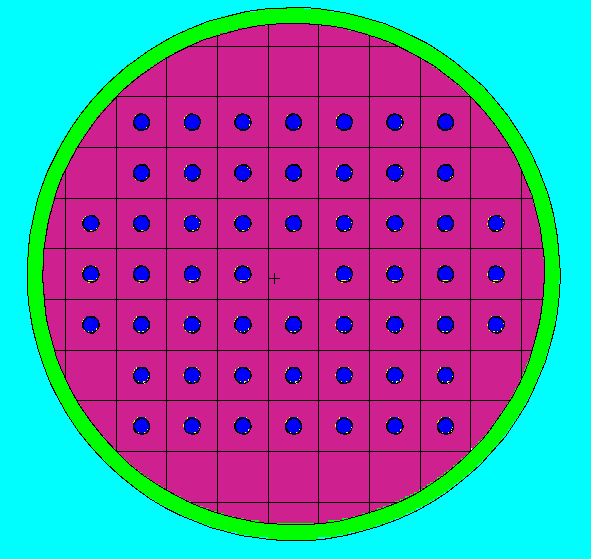
\includegraphics[width=4in]{../images/hetero_xy.png}
\caption{Heterogeneous reactor model for validating homogeneous geometry
approximations}
\label{fig:hetero_xy}
\end{figure}


\begin{table}[h]
  \centering
  \caption{Results of homogeneous geometry validation}
  \begin{tabular}{lll}
    \toprule
     Model                             & \keff & stdv       \\
    \midrule
     Homogeneous              		   & 1.13777 & 0.00013  \\
     Heterogeneous 					   & 1.13159 & 0.00013  \\
  \end{tabular}
  \label{tab:homog_validate_results}
\end{table}

\section{Depletion Verification}
